\section{Einleitung}

Diese Arbeit befasst sich mit der Evaluation der Theorie, den Standards und Protokollen, ausgewählten Produkten, den Risiken und den Geschäftsmodellen, welche sich hinter dem Schlagwort \glqq Smart Home\grqq \ einreihen.
Ziel ist es, auch mit Hilfe der Methoden der Systemanalyse, mit falschen Vorstellungen aufzuräumen, den aktuellen Stand der Dinge darzulegen und einen Blick in die Zukunft der intelligenten Gebäude zu werfen.

\subsection{Definition: Smart Home}

Es existiert keine eindeutige Definition für Smart Homes.
Häufig wird unter Smart Home ein System verstanden, welches die Fähigkeit besitzt Beleuchtung, Temperatur, Zugang zum Gebäude und Unterhaltungsgeräte, wie z.B. ein Fernseher, über eine Schnittstelle zu kontrollieren.
\autoref{fig:smart_home_devices} zeigt eine Reihe möglicher Komponenten eines Smart Home Systems.

\begin{wrapfigure}{r}{0.5\textwidth}
	\centering
	\caption{Smart Home Komponenten}
	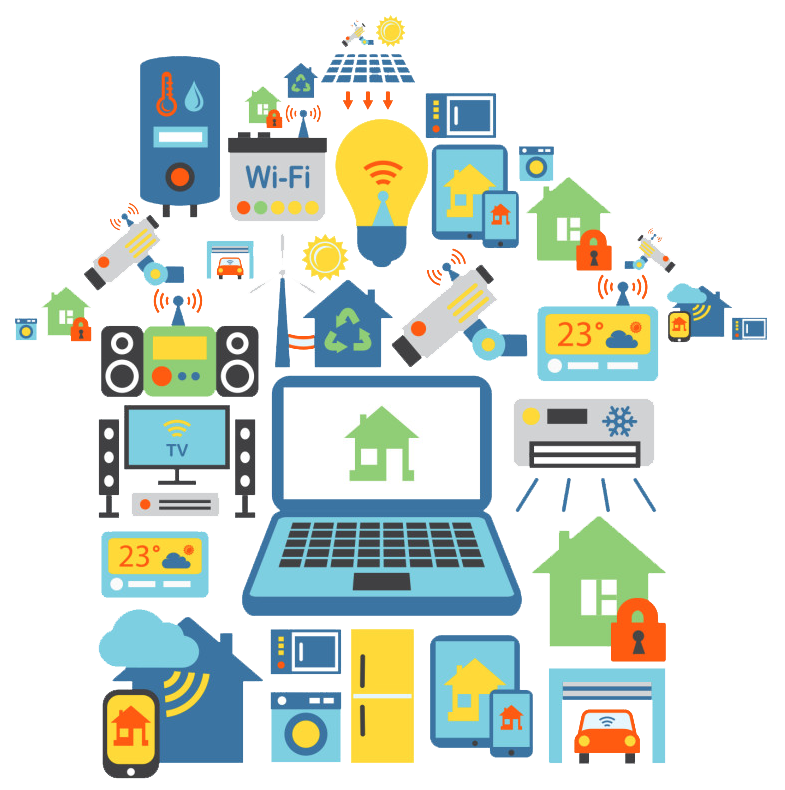
\includegraphics[width=0.45\textwidth]{smart-home}
	\caption*{\footnotesize{Quelle: \mycite[Vgl.][]{figure_smart_home}}}
	\label{fig:smart_home_devices}
\end{wrapfigure}

Oft werden bei Smart Home Systemen auch alle Geräte mit einem zentralen sog. \glqq Hub\grqq \ verbunden, welcher die Nutzung verschiedener Komponenten auf Ressourcenschonung optimiert und automatisiert.
So werden Smart Home Systeme oft mit Energieeinsparungen beworben, welche sich daraus ergeben, dass z.B. nur geheizt wird, wenn auch Menschen anwesend sind.
Auch Komfortfunktionen, welche auf Automatisierungen, wie etwa dem automatischen Anschalten einer Zimmerlampe, wenn das Zimmer nicht mehr hell genug ausgeleuchtet ist und ein Mensch anwesend ist, werden oft zur Schau gestellt.\myfootcite[Vgl.][]{smart_home_def_usa,smart_home_def_cnbc}

Aschendorf erkennt in jedem Smart Home verallgemeinernd die Verbindung von Geräten, Automatisierungen und die Kontrolle über die verbundenen Geräte als elementare Bestandteile eines Smart Homes.\myfootcite[Vgl.][59ff]{aschendorf14}

Des Weiteren ist sogar der Begriff \glqq Smart Home\grqq \ nicht überall in Gebrauch. Im englischsprachigen Raum ist der Begriff \glqq Home automation\grqq \ (zu Deutsch \glqq Heimautomatisierung\grqq ) geläufig.
Auch \glqq Domotics\grqq \ (vom lateinischen Wort \glqq domus\grqq \ für \glqq Haus\grqq ) kann synonym genutzt werden.\myfootcite[Vgl.][]{smart_home_def_hill}

\subsection{Geschichte}

Als zu Beginn des 20. Jahrhunderts erste Haushaltsgeräte wie Kühlschrank oder Staubsauger erfunden wurden entstand gleichzeitig der Wunsch, dass die Geräte ihre Aufgaben auch autonom und in Absprache erledigen könnten.\myfootcite[Vgl.][]{smart_home_history_iotevolutionworld}

Erst 1966 hat Jim Sutherland dann den ersten Smart Home Prototypen im heutigen Sinne entworfen und in Betrieb genommen - den \ac{ECHO} IV.
Der \ac{ECHO} IV fungierte damals als Wecker, Fernbedienung für den Fernseher und die Musikanlage und als Uhr.
Sutherland plante auch mit dem \ac{ECHO} IV die hauseigene Beleuchtung zu steuern.\myfootcite[Vgl.][]{smart_home_history_echoiv}

Nachdem 1970 die ersten Mikrocomputer von Pico entwickelt wurden, beschäftigte sich Pico unter dem Projekt X10 mit der Idee Beleuchtung und andere Haushaltsgeräte über deren Stromkabel anzusteuern.
1978 wurde das Projekt unter dem Produktnamen X10 (später X10 Powerhouse).
Weitere Iterationen des Smart Home Systems wurden bis heute vertrieben.\myfootcite[Vgl.][]{smart_home_history_x10}

\begin{figure}[ht]
	\centering
	\caption{Google Trends zu Smart Home}
	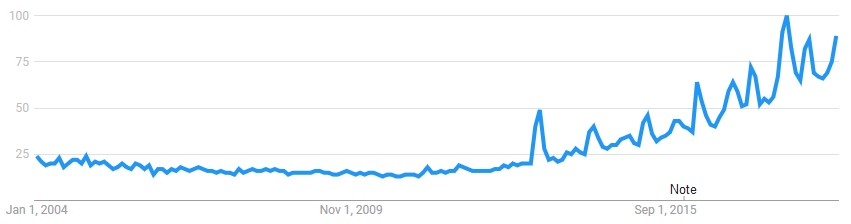
\includegraphics[width=0.9\textwidth]{smart-home-google-trends}
	\caption*{\footnotesize{Quelle: \mycite{google_trends_smart_home}}}
	\label{fig:googletrendssmarthome}
\end{figure}

Ohne einen stärkeren Trend verzeichnen zu können wurden einzelne Haushaltsgeräte immer weiter optimiert und digitalisiert.
2012 veröffentlichte ABI Research, dass im besagten Jahr 1,5 Millionen Smart Home Systeme in den USA installiert wurden - 50\% mehr als im Jahr zuvor.\myfootcite[Vgl.][]{smart_home_history_market2012}
Dieser Trend setzte sich bis heute fort, auch weil im selben Jahr Amazon Alexa vorgestellt wurde, was das Thema Smart Home normalen Konsumenten näher brachte.\myfootcite[Vgl.][]{alexa_release}
\autoref{fig:googletrendssmarthome} zeigt die Popularität des Trends Smart Home seit 2004, gemessen anhand Google-Suchanfragen.
Je höher der Wert auf der Y-Achse, desto populären war der Trend, relativ im Vergleich du allen anderen Suchanfragen.\myfootcite[Vgl.][]{google_trends_docs}

\subsection{Internet of Things}

Das \ac{IoT} hat zunächst nichts mit Heimautomatisierung zu tun.
Unter dem Internet der Dinge versteht man grundlegend die Verbindung von Geräten untereinander, sowie mit dem Internet.\myfootcite[Vgl.][]{ibm_iot}
Durch die Verbindung verschiedener Geräte, wie etwa einer Lichtschranke und einer Glühbirne, kann Mehrwert für den Benutzer der Geräte geschaffen werden, indem z.B. die Glühbirne automatisch bei Aktivierung der Lichtschranke aktiviert wird.
Zu einer Anwendung des \acp{IoT} wird das Beispiel, wenn das Internet noch mit involviert wird.
So wären hier Benachrichtigungen zu Bewegungsmeldungen oder Steuerung der Glühbirne über das Internet denkbar.

Ein Smart Home System kann also zum \ac{IoT}-System werden, wenn die Steuerung oder Automatisierung über eine Instanz im Internet abgewickelt wird.
Dies muss jedoch nicht der Fall sein.
So stellt die Software Home Assistant z.B. die Möglichkeit ein Smart Home System komplett offline zu betreiben.\myfootcite[Vgl.][]{hass_vision}

\section{Evaluation}

Folgend wird das Smart Home von Grund auf durchdacht, die zugehörigen technischen Elemente vorgestellt und schließlich Beispiele betrachtet.
Anhand dieser werden dann auch die Risiken beim Betreiben eines Smart Home Systems greifbar.
Anschließend werden Auswahl an Geschäftsmodellen vorgestellt, welche vorhergehende Erläuterungen monetarisieren.

\newpage

\subsection{Aufbau eines Smart Home Systems}\label{sec:aufbau}

Aschendorf beschreibt den Aufbau von Smart Home Systemen als stufenförmige Hierarchie.
\autoref{fig:automatisierungspygramide} zeigt die drei Ebenen der Automatisierungspyramide nach Aschendorf:
Die Feldbusebene, die Automatisierungsebene und die Leitebene. \myfootcite[Vgl.][59]{aschendorf14}

\begin{figure}[ht]
	\centering
	\caption{Automatisierungspyramide nach Aschendorf}
	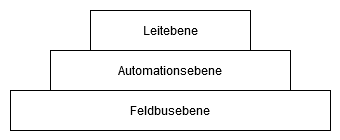
\includegraphics[scale=0.8]{Automatisierungspyramide_nach_Aschendorf}
	\caption*{\footnotesize{Quelle: Eigene Darstellung.}}
	\label{fig:automatisierungspygramide}
\end{figure}

\subsubsection{Feldbusebene}

Die Feldbusebene besteht aus sämtlichen eingebauten Systemkomponenten, also Gateways, welche verschiedene Systeme verbinden, Sensoren, welche z.B. Temperatur und Luftfeuchtigkeit überwachen, und Aktoren, wie z.B. Glühbirnen.
In der selben Ebene finden sich auch die Verbindungen der oben genannten Geräte wieder.
So ist die Feldbusebene in sich bereits funktional und direkt nutzbar.
Es kann z.B. der Sensor \textit{Lichtschalter 3} ausgelöst werden, welcher den Aktor \textit{Deckenlampe Wohnzimmer} aktiviert.\myfootcite[Vgl.][66-67]{aschendorf14}

\subsubsection{Automatisierungsebene}

Geräte übergreifende Automatisierungen werden in der Automatisierungsebene implementiert.
Dies wird durch einfache Controller oder programmierbare Mikrocomputer realisiert.
Nach der Änderung von Zuständen, wie z.B. der aktuellen Zeit, die Anwesenheit eines Bewohners oder die Temperatur eines Raumes, passt sich das Smart Home System mit dieser zusätzlichen Ebene nun nach vorgegebenen Regeln autonom an.\myfootcite[Vgl.][67-68]{aschendorf14}

\subsubsection{Leitebene}

Die Leitebene widmet sich der Interaktion des Smart Home Systems mit dessen Bewohnern.
Es lässt sich die Interaktion teilen in Eingaben und Ausgaben.
Zu den Eingaben zählen Befehle, die z.B. über Steuerungs-Apps gesendet werden oder von einem zentralen Steuerungscomputer emittiert werden.
Ausgaben werden etwa über digitale Dashboards auf diversen Displays angezeigt.
Über dieselben werden meist auch Fehlerdiagnosemeldungen angezeigt.\myfootcite[Vgl.][68-70]{aschendorf14}

\subsection{Verbindungssysteme}

In einem Smart Home System kommen Produkte verschiedener Art zum Einsatz.
Vom digitalen Kühlschrank, zum Türschloss hin zu Lichtschalter und Glühbirne.
Aufgrund der verschiedenenartigen Anwendungen der Produkte und den verschiedenen Herstellern werden im Smart Home Bereich verschiedene Verbindungssysteme und Protokolle verwendet.
Nachfolgend wird eine Auswahl der geläufigsten Systeme vorgestellt.

\subsubsection{LAN und WLAN}

2017 verfügten nach dem Statistischen Bundesamt 85,9\% aller deutschen Haushalte über einen stationären Internetzugang und damit einhergehend ein privates \ac{LAN} oder \ac{WLAN}.\myfootcite[Vgl.][]{haushalte}
Deshalb wird bei der nachträglichen Installation eines Smart Home Systems häufig auf \ac{LAN} oder \ac{WLAN} zurückgegriffen um Kosten und Installationsaufwand einzusparen.

Ein \ac{LAN} wird durch einen oder mehrere sog. Switches über Ethernet-Kabel verbunden.
Alternativ kann auch ein Router anstelle der Switches verwendet werden.
Dieser kann das \ac{LAN} sogar zusätzlich mit anderen \acp{LAN} verbinden, bspw. mit dem Internet.
Beim \ac{WLAN} wird an Stelle der Ethernet-Kabel über das 2,4 oder 5 GHz Band gefunkt.\myfootcite[Vgl.][]{local_area_network}

\autoref{fig:yeelight} zeigt die LED-Lampe \glqq Yeelight LED Bulb\grqq \ von Xiaomi, ein für Smart Home System Nachrüstungen gut geeignetes Produkt.
Die LED-Lampe nutzt das \ac{WLAN} zur Kommunikation mit der Steuerungskomponente und die vorhandene E27 Fassung zur Stromversorgung.\myfootcite[Vgl.][]{yeelight_wifi_bulb}

\begin{wrapfigure}{r}{0.4\textwidth}
	\centering
	\caption{Yeelight Glühbirne}
	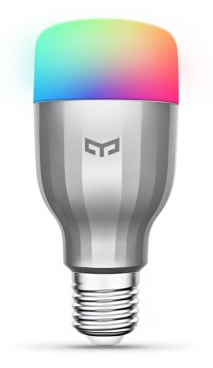
\includegraphics[scale=.45]{yeelight-bulb}
	\caption*{\footnotesize{Quelle: \mycite{figure_yeelight}}}
	\label{fig:yeelight}
\end{wrapfigure}

Der Einsatz von einem \ac{LAN} als Kommunikationssystem für Smart Home Anwendungen ist jedoch nicht uneingeschränkt zu empfehlen.
So sollte bedacht werden, dass die Integration eines beliebigen Smart Home Produkts Sicherheitslücken mit in das private \ac{LAN} reißen kann.
Bspw. könnte über das Ethernet-Kabel zu einer außen am Haus montierten Überwachungskamera auf das gesamte Heimnetzwerk zugegriffen und mitgelauscht werden.

\subsubsection{MQTT}

\ac{MQTT} ist ein speziell auf das \ac{IoT} ausgerichtetes Netzwerk-Protokoll.

\begin{figure}[ht]
	\centering
	\caption{MQTT Beispiel}
	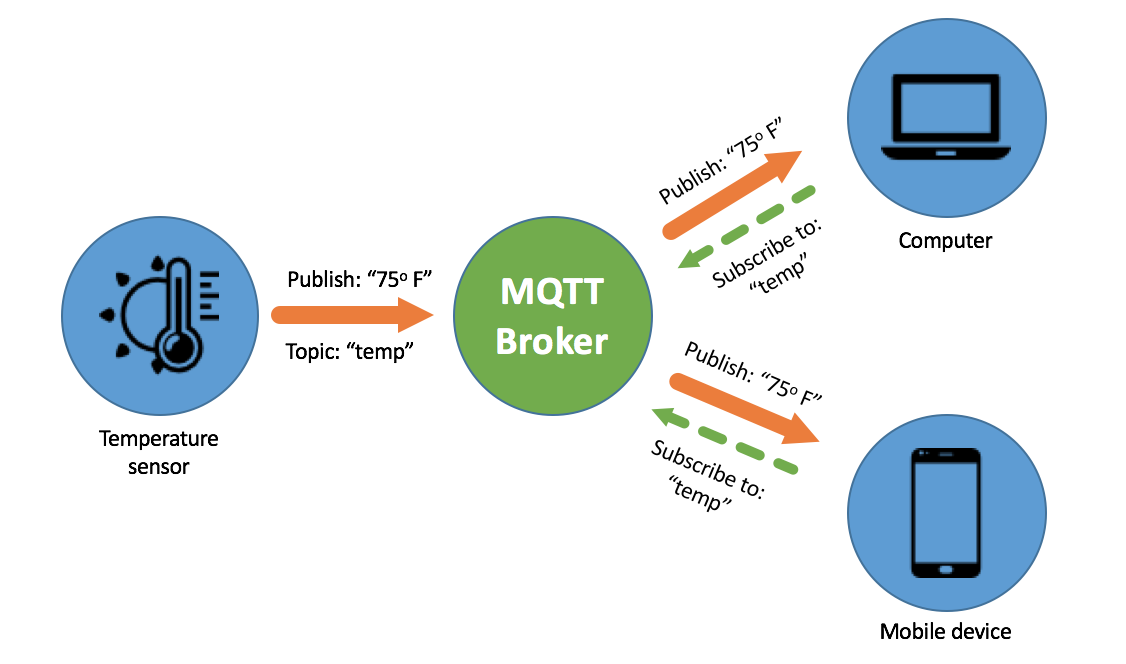
\includegraphics[scale=.4]{mqtt-example}
	\caption*{\footnotesize{Quelle: \mycite{figure_mqtt_architecture}}}
	\label{fig:mqtt_example}
\end{figure}

Anhand \autoref{fig:mqtt_example} lässt sich die Funktionsweise von \ac{MQTT} erklären.
Es gibt einen zentralen Server, den sog. Broker, über welchen diverse Geräte (die Clients) kommunizieren.
Dabei gibt es zwei Methoden:
Ein Client kann Daten zum Broker zu einem angegeben Thema senden und ein Client kann einem Broker mitteilen zu einem Thema informiert werden zu wollen.
Trifft eine Nachricht bei einem Broker ein schaut dieser nach, ob ihm zu dem entsprechenden Thema Abonennten bekannt sind und leitet ggf. die Nachricht weiter.
Kommunikation in \ac{MQTT} also nach dem Push-Prinzip statt, d.h. ein Client sendet keine Anfragen sondern erhält bei einem Ereignis eine Benachrichtigung.
Umgekehrt verfährt z.B. das \ac{HTTP}.
Zusätzlich garantiert \ac{MQTT} die Übermittlung einer Nachricht.
Bei Verbindungsabbruch oder Beschädigung der Nachricht wird die Nachricht weiter gesendet, bis das Senden erfolgreich verläuft.
Ebenso kann garantiert werden, dass eine Nachricht nur ein einziges Mal den Empfänger erreicht.\myfootcite[Vgl.][1]{mqtt_docs}

Anwendung findet das \ac{MQTT} Protokoll vor allem bei Sensoren für Raumtemperatur, Lichteinfall oder Bewegung, da hier eine lediglich eine eindimensionale Kommunikation abgebildet werden muss.
Da \ac{MQTT} ein offener und frei verfügbarer Standard ist, findet sich das Protokoll auch vermehrt in \ac{DIY}-Projekten wieder.\myfootcite[Vgl.][]{bruhautomation_esp_sensor}

Für die Nutzung von \ac{MQTT} spricht oft die Architektur des Protokolls, welche über den Broker das Senden von Nachrichten von vielen an viele ermöglicht.
Andererseits muss abgewägt werden, dass \ac{MQTT} auf Protokollebene keine Verschlüsselung nutzt.
Es können zwar auf höherer Ebene Sicherheitsfunktionen implementiert werden, jedoch würden diese die Geschwindigkeit des \ac{MQTT}-Protokolls signifikant verringern.\myfootcite[Vgl.][]{mqtt_pros_cons}

\subsubsection{ZigBee}

\begin{wrapfigure}{r}{0.35\textwidth}
	\centering
	\caption{ZigBee Stack}
	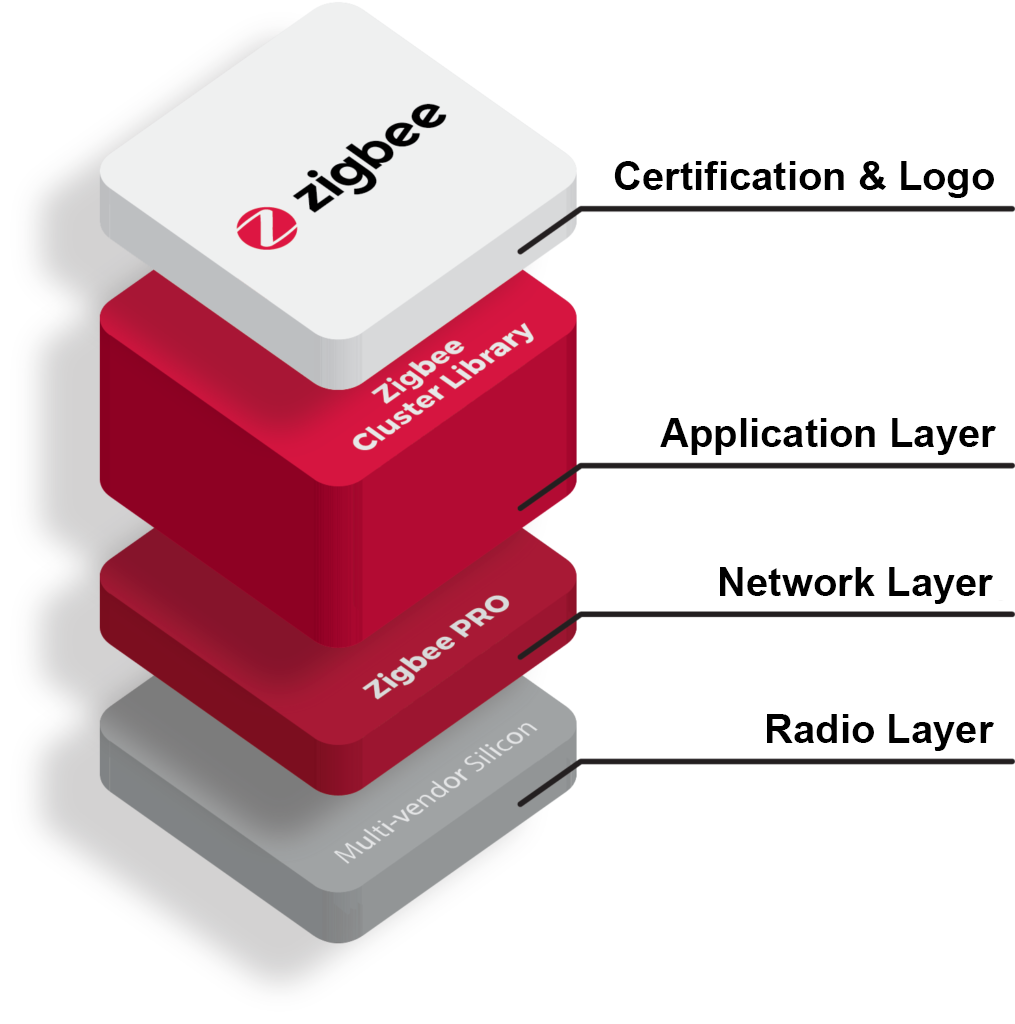
\includegraphics[width=0.35\textwidth]{zigbee-stack}
	\caption*{\footnotesize{Quelle: \mycite[Vgl.][]{figure_zigbee_stack}}}
	\label{fig:zigbee_stack}
\end{wrapfigure}

ZigBee ist eine Komplettlösung für das \ac{IoT}.
\autoref{fig:zigbee_stack} zeigt ZigBees Aufbau.
Die unterste Ebene stellt den Standard IEEE 802.15.4 dar - ein Übertragungsprotokoll für die untersten Ebenen eines \ac{WPAN}.
Auf dieser Ebene basiert die niedrigste Ebene ZigBees, die Netzwerkebene ZigBee PRO.
Diese ist global nutzbar, da das 2,4 GHz Band nach IEEE 802.15.4 definiert genutzt wird.
Die kennzeichnende Eigenschaft von ZigBee PRO ist jedoch die Vernetzung von Geräten, welche nicht nur schnell, sondern auch dezentral erfolgt.
So wird eine Nachricht etwa von einer Glühbirne, zu einer Steckdose, über einen Kühlschrank hin zu dem sog. ZigBee Hub gesendet, welches die Schnittstelle zur Interaktion mit ZigBee Geräten darstellt und somit die Reichweite und Signalstärke des ZigBee Netzwerkes erhöht.
Darüber hinaus implementiert ZigBee PRO Energiesparmechanismen, welche im Smart Home Sektor mit vielen Batterie betriebenen Geräten nützlich sind.
Ebenso liefert ZigBee PRO \ac{MQTT}-ähnliche Übertragungsarten, sowie eine Verschlüsselung der Kommunikation nach \ac{AES}.
Schließlich bietet die \ac{ZCL}, welche auf ZigBee PRO basiert, Entwicklern die Möglichkeit ZigBee einfach in eine beliebige Anwendung zu integrieren.
Die ZigBee-Zertifizierung eines Geräts stellt abschließend sicher, dass weitere Geräte nach ZigBee Spezifikation mit dem Gerät interagieren können.\myfootcite[Vgl.][]{zigbee_faq}

Der Beleuchtungssystemanbieter Signify nutzt ZigBee um Philips Hue Beleuchtungssyteme zuverlässig und kabellos zu installieren.
Gerade bei Gebäuden mit vielen massiven Wänden kann es von Vorteil sein ein \ac{P2P} System zu verwenden um ein Netzwerk aufzubauen, da zentrale Router nicht unbedingt alle Ecken eines Gebäudes abdecken können.\myfootcite[Vgl.][]{how_hue_works}

Für die Nutzung von ZigBee spricht vor allem die Interoperabilität zwischen verschiedenen ZigBee Geräten, welche durch die Zertifizierung und das global nutzbare 2,4GHz Band sichergestellt werden.
Damit werden ZigBee Systeme nicht nur einfach zu programmieren, sondern für Konsumenten auch einfacher zu installieren.
Die Möglichkeit \ac{P2P}-Netzwerke mit ZigBee Geräten zu bilden sorgt zudem für eine bessere Verbindung der einzelnen Geräte.
Schließlich können zusätzlich Batterie betriebene Geräte von ZigBees geringem Stromverbrauch profitieren.\myfootcite[Vgl.][]{zigbee_faq}

Es ist jedoch keine uneingeschränkte Empfehlung für ZigBee auszusprechen.
ZigBee ist zwar ein offener Standard, jedoch nicht kompatibel mit u.a. der \ac{GPL}.
Dies hat zur Folge, dass ZigBee nicht in freie Software implementiert werden kann.\myfootcite[Vgl.][]{iot_standard_war}
Außerdem besteht die Hürde eines jährlich zu entrichtenden Mitgliedsbeitrags um Zugang zu den ZigBee Spezifikationen und Standards zu erhalten, was Hobby-Programmierer und Bastler fern von ZigBee hält.\myfootcite[Vgl.][]{zigbee_membership}
Des Weiteren können herkömmliche Smartphones und Tablets nicht mit in ein ZigBee Netzwerk integriert werden, da diese nicht über den benötigten ZigBee Stack verfügen.
So muss immer ein ZigBee Hub installiert werden, welches die Schnittstelle zu herkömmlichen Systemen wie \ac{LAN} und \ac{WLAN} bildet.
Abschließend bleibt anzumerken, dass aufgrund der \ac{P2P}-Architektur ZigBees maximal Datenübertragungsraten von bis zu 250 kbit/s erreicht werden.\myfootcite[Vgl.][]{zigbee_faq}

\subsubsection{Z-Wave}

Z-Wave lässt sich nahezu identisch wie ZigBee beschreiben.\myfootcite[Vgl.][]{zwave_faq}
So wird auch eine \ac{P2P} Mesh Netzwerk-Topologie genutzt.

\begin{figure}[ht]
	\centering
	\caption{Star- vs. Mesh-Netzwerk}
	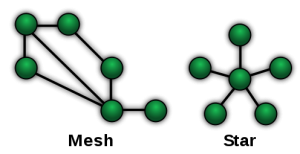
\includegraphics[scale=0.9]{star-vs-mesh-network}
	\caption*{\footnotesize{Quelle: \mycite{figure_star_vs_mesh_network}}}
	\label{fig:star_vs_mesh_network}
\end{figure}

\autoref{fig:star_vs_mesh_network} vergleicht die \ac{P2P} Mesh-Topologie mit der klassischen Stern-Topologie, wie sie z.B. bei einem \ac{WLAN} zu finden ist.
Bei einer Stern-Topologie sind alle Geräte im Netzwerk mit einem zentralen sog. Router verbunden, welcher die Nachrichten der Geräte einander entsprechend weiterleitet.
Bei einer Mesh-Topologie hingegen verbinden sich die Geräte mit allen Geräten in ihrer Reichweite.
Eine Nachricht an ein bestimmtes Gerät wird nun von Gerät zu Gerät geschickt, bis das empfangende Geräte das Empfänger-Gerät ist.
Hier müssen jedoch im Vergleich zur Stern-Topologie Abstriche bzgl. der Latzenz einer Nachricht gemacht werden, da eine Nachricht selten über eine direkte Verbindung gesendet werden kann.
Andererseits kann ein Mesh-Netzwerk einfacher expandiert werden, da jedes Gerät im Netzwerk Teil des Netzwerks ist.

\begin{wrapfigure}{r}{0.35\textwidth}
	\centering
	\caption{Z-Wave Chip}
	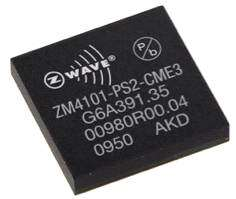
\includegraphics[width=0.2\textwidth]{zwave-chip}
	\caption*{\footnotesize{Quelle: \mycite{figure_zwave_chip}}}
	\label{fig:zwave_chip}
\end{wrapfigure}

Auch was den Energiebedarf eines Z-Wave Netzwerks anbelangt, kann kein Unterschied zu ZigBee festgestellt werden.
Beide Systeme ermöglichen es Batterie betriebenen Geräten über mehrere Jahre Nachrichten zu senden und zu empfangen, ohne Batterie-Wechsel.\myfootcite[Vgl.][]{smartcave_zwave_vs_zigbee}

Im Gegensatz zu ZigBee ist Z-Wave kein offener Standard.
So wird beim Bau eines Z-Wave kompatiblen Geräts ein proprietäres Bauteil benötigt.
\autoref{fig:zwave_chip} zeigt einen Z-Wave Funksendeempfänger von Sigma Designs aus 2012.
Dass die Hersteller von Z-Wave Geräten den Z-Wave Funksendeempfänger fremdbeziehen müssen bedeutet auf der einen Seite, dass Fehler im Z-Wave Funksendeempfänger nicht vom Hersteller korrigiert werden können und so evtl. Geräte zurückgerufen werden müssen, andererseits wird so sichergestellt, dass kein Hersteller das Herz eines jeden Z-Wave Geräts, die Kommunikationseinheit, verändert und somit die Interoperabilität aller Z-Wave Geräte nicht gefährden kann.\myfootcite[Vgl.][]{zwave_develop_a_product}

\begin{table}[ht]
	\caption{Z-Wave und ZigBee im Vergleich}
	\centering
	\begin{tabular}{| p{0.4\textwidth} | p{0.3\textwidth} | p{0.2\textwidth} |}
		\hline
		\textbf{Merkmal} 	& \textbf{Z-Wave} & \textbf{ZigBee} \\ \hline
		Kompatible Geräte & 2400+ & 2500+ \\ \hline
		Beteiligte Firmen & 418 & 322 \\ \hline
		Anzahl verkaufter Produkte & 100+ Mio.& 300+ Mio.\\ \hline
		Netzwerk-Topologie & Mesh & Mesh \\ \hline
		Max. Anzahl an Geräten im Mesh & 232 & ca. 65000 \\ \hline
		Genutzte Frequenzen & u.a. 868,4 MHz (EU); 908,4 MHz (US) & 2,4 GHz \\ \hline
	\end{tabular}
	\caption*{\footnotesize{Quellen: \mycite[Vgl.][]{zwave_product_count,zigbee_faq,zwave_member_count,safewise_zwave_vs_zigbee,zwave_faq,smartcave_zwave_vs_zigbee,zwave_frequencies,zigbee_member_count,zwave_products_sold}}}
	\label{tab:zwave_vs_zigbee}
\end{table}

Noch kann nicht abgeschätzt werden, ob sich Z-Wave oder ZigBee oder ein dritter \ac{IoT}-Standard durchsetzen wird.
Nach \autoref{tab:zwave_vs_zigbee} sind Z-Wave und ZigBee was beteiligte Firmen, kompatible Geräte und verkaufter Produkte angeht nahezu gleichauf.
Auf technischer Ebene sind die Standards zwar ähnlich, nicht aber gleich.
So kann mit ZigBee bspw. ein größeres Mesh-Netzwerk erstellt werden.
Hauptsächlich relevant beim Z-Wave-ZigBee-Vergleich sind jedoch die genutzten Frequenzen.
Da ZigBee das 2,4 GHz Band mit anderen Technologien wie z.B. \ac{WLAN} teilt, muss ZigBee mit Interferenzen operieren, während Z-Wave weitestgehend ungestört operieren kann.
Außerdem kann Z-Wave durch die geringere Frequenzen eine höhere Signalreichweite erzielen.
ZigBee hingegen erreicht durch die höhere Frequenz eine höhere Bandbreite.
Schließlich kann ZigBee auch wegen der globalen Nutzung der 2,4 GHz Frequenz regional limitiert kompatible Produkte vermeiden.
Z-Wave hingegen nicht.\myfootcite[Vgl.][]{zwave_faq}

\subsection{Risiken}

Um Risiken beim Betrieb eines Smart Home Systems erkennen zu können, muss zunächst verstanden werden, auf welche Faktoren diese sich beziehen können.
Zuerst sind hier die persönlichen Daten der Bewohner eines Smart Home Systems zu nennen.
Durch jede Interaktion mit dem System fallen zwangsweise Daten an.
So ist einem Smart Home System bspw. bekannt wann sich seine Bewohner in welchem Raum aufhalten, wann sie schlafen oder wann sie sich außer Haus aufhalten.
Die restlichen drei von Risiken behafteten Faktoren ergeben sich aus dem Aufbau eines Smart Home Systems, wie in \autoref{sec:aufbau} beschrieben.
Aus der Leitebene leitet sich der Faktor Kontrolle ab, aus der Automatisierungsebene Automatisierungen und schließlich grundlegende Vernetzung aus der Feldbusebene.

Das primäre Risiko welches sich aus den vorhandenen Daten ableitet kann als unautorisierter Zugriff durch Dritte beschrieben werden.
So sollten die üblichen Aufenthaltszeiträume der Bewohner eines Smart Home Systems nicht für potentielle Einbrecher abrufbar sein.
Auch ist fraglich auf welche Daten die beteiligten Anbieter von Smart Home Komponenten zugreifen dürfen.

Kontrollverlust oder ungewollte Kontrolle sind Ausprägungen des Risikofaktors Kontrolle.
So ist sicher nicht gewollt, dass durch eine Systemstörung bei einem Anbieter einer Smart Home Komponente diese nicht mehr steuerbar wird.
Ebenso sollten Dritte sicherheitsrelevante Komponenten, wie etwa Türen und Fenster, nicht kontrollieren dürfen.

Auch leuchtet ein, dass Automatisierungen nicht ausfallen sollten.
So könnte z.B. Energie verschwendet werden, wenn Temperatursensoren, Anwesenheitssensoren und die Heizungssteuerung sich nicht mehr automatisch abstimmen können.

Schließlich bleibt zu klären, dass Störungen der grundlegenden Vernetzung der einzelnen Komponenten fatale Risiken mit sich bringen können.
Bei einem Stromausfall könnte so z.B. das Öffnen einer Türe nicht mehr möglich sein, wenn die Vernetzung des Türschlosses und einem Anwesenheitssensor nicht mehr funktional ist.

\subsubsection{Schwachstellen}

Sollen Schwachstellen eines Smart Home Systems erkannt werden muss zunächst geklärt werden, ob es sich um ein Smart Home System mit \ac{IoT}-Funktionalitäten handelt.

Wird ein Smart Home System lokal betrieben und die Fernsteuerung über ein \ac{VPN} realisiert können Angriffe aus dem Internet weitgehend ausgeschlossen werden.
Die Schwachstellen eines lokalen Systems befinden sich primär an den von außerhalb des Gebäudes erreichbaren Geräten.
So kann sich bspw. über eine außen am Gebäude angebrachte Überwachungskamera Zugang ins Heimnetzwerk verschafft werden, indem etwa das Netzwerkkabel, welches die Kamera mit dem Heimnetzwerk verbindet, direkt angezapft wird.
Auch Sprachassistenten können von außen angesteuert werden, was einem Angreifer bspw. ermöglichen würde, sich mit dem lauten Rufen von \glqq Alexa, öffne die Haustüre!\grqq \ Zugang zum Gebäude zu verschaffen.
Schließlich ist ein Smart Home System jeder Art abhängig von einer konstanten Stromversorgung.
Bei einem Stromausfall kann ein Smart Home System an Funktionalität jeglicher Art verlieren.

Ist ein Smart Home über ein Hub oder mehrere einzelne Geräte direkt mit dem Internet verbunden ergeben sich weitere Lücken.
Zunächst sollte bewusst sein, dass die eigenen Daten sich nicht mehr unter eigener Kontrolle befinden, sobald \ac{IoT}-Komponenten genutzt werden, was bedeutet, dass Dritte verantwortlich für die Sicherheit der eigenen Daten sind.
Meist wird nicht klar kommuniziert, wie die eigenen Daten verarbeitet und gespeichert werden.
Auch wird es teilweise erst verzögert bekannt gegeben, wenn Daten abhanden gekommen sind, bzw. die Systeme Dritter offene Lücken hatten.
So ergibt sich eine unvermeidbare und unkontrollierbare Schwachstelle beim Einsatz von \ac{IoT}-Geräten.
Darüber hinaus werden \ac{IoT}-Geräte dem Internet oft direkt ausgesetzt, was zur Folge hat, dass Dritte sich über eben diese Geräte Zugriff auf ein Smart Home System verschaffen können, weil \ac{IoT}-Geräte oft nicht richtig konfiguriert sind, oder Sicherheitslücken aufweisen, welche nicht vom Hersteller geschlossen werden.\myfootcite[Vgl.][]{iot_software_problem}

\subsubsection{Risikoprävention}

Präventive Maßnahmen leiten sich direkt aus den genannten Schwachstellen ab.
Generell empfiehlt sich der Verzicht auf \ac{IoT}-Systeme, wie Amazon Alexa, was die Abhängigkeit von Dritten reduziert.
Werden trotzdem \ac{IoT}-Komponenten eingesetzt, sollte deren Zugang ins Internet über eine Firewall möglichst beschränkt werden.
Auch kann versucht werden die Komponenten lokal anzusprechen und den Zuganz zum Internet gänzlich zu sperren.
Oft verfügen \ac{IoT}-Geräte über eine \ac{API}, welche direkt angesprochen werden kann.
Xiaomi erlaubt z.B., dass ihre Yeelight Lampen über ein \ac{IoT}-System per App, aber auch direkt über das \ac{LAN} steuerbar sind.\myfootcite[Vgl.][]{yeelight_docs}

Ein Stromausfall und somit ein genereller Systemausfall kann durch einen Heimspeicher für elektrische Energie kompensiert werden.
Zusätzlich sollten kritische Funktionen, wie etwa die Verriegelung von Türen, auch ohne Strom und Internet nutzbar sein - es sollten also Rückfalleinrichtungen vorhanden sein.
Die Bedeutung von Rückfalleinrichtungen wird bewusst, wenn z.B. der Ausfall von Lockstate Smart Home Türschlössern im August 2017 rekapituliert wird.
Ca. 500 Kunden von Lockstate konnten ihre Türen nicht mehr öffnen, weil eine fehlerhafte Aktualisierung der Software der Schlösser deren Funktionalität deaktivierte.\myfootcite[Vgl.][]{iot_fail}

Die Risiken der Sprachsteuerungseinheiten können entschärft werden, indem man die Berechtigungen der Spracheingaben so definiert, dass lediglich nicht sicherheitsrelevante Aktion ausgeführt werden können.
So kann man bspw. den Befehl \glqq Alex, schließe die Haustüre!\grqq \ erlauben, den Befehl \glqq Alex, öffne die Haustüre!\grqq \ aber verbieten.

Schließlich bleibt zu empfehlen alle von außen zu erreichende Geräte in einem separaten Netzwerk zu organisieren, damit nicht auf das interne Netzwerk von außen zugegriffen werden kann.

\subsection{Produkte}

Folgend wird eine repräsentative Auswahl an Smart Home Systemen vorgestellt und eingeordnet.
Amazon Alexa repräsentiert die Nachrüstungslösung, welche auch mit wenig technischem Verständnis installiert werden kann, das Open Source Projekt Home Assistant die universale Bastlerlösung und schließlich HomeMatic IP das Smart Home Komplettsystem mit Option zur professionellen Unterstützung.

\subsubsection{Amazon Alexa}

\begin{figure}[ht]
	\centering
	\caption{Alexa Geräte}
	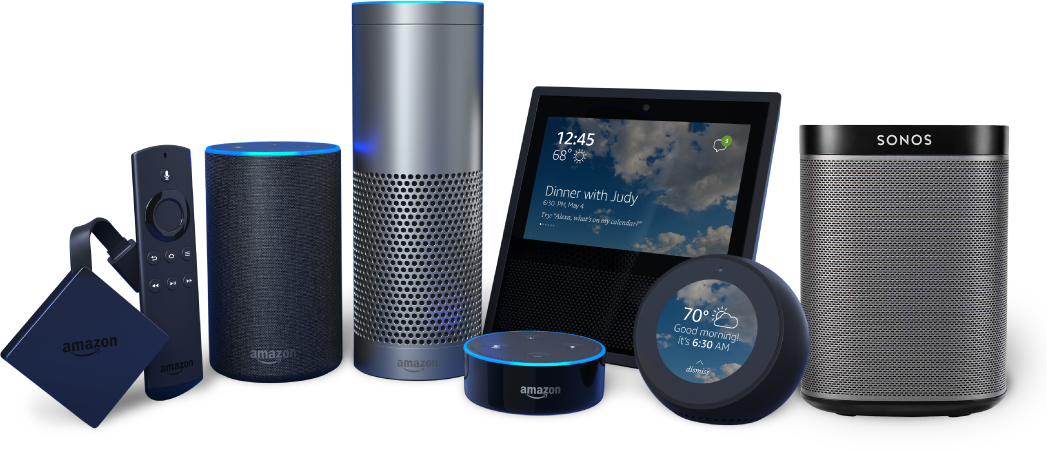
\includegraphics[width=.8\textwidth]{alexa_devices}
	\caption*{\footnotesize{Quelle: \mycite{figure_alexa_devices}}}
	\label{fig:alexa_devices}
\end{figure}

Amazon Alexa ist die Software für einen intelligenten Sprachassistenten, bestehend aus einem Lautsprecher, einem Mikrofon sowie einer Internetanbindung, welche seit 2014 in Alexa Geräten, wie in \autoref{fig:alexa_devices}, verbaut wird.\myfootcite[Vgl.][]{alexa_release}
Über die Internetanbindung wird auf ein Amazon Rechenzentrum zugegriffen, in welchem Ressourcen für die Verarbeitung von Spracheingaben mit \ac{ASR} und \ac{NLU} bereitgestellt werden.

Unter \ac{ASR} versteht man die Umwandlung von menschlicher Sprache in Text.
Die Auslagerung der Rechenleistung in die Cloud sorgt für eine Beschleunigung der \ac{ASR}, sodass nahezu keine Latenz zu bemerken ist.\myfootcite[Vgl.][]{alexa_asr}

Lokal ist eine weitere \ac{ASR} Einheit verbaut, welche im Betrieb nach dem Stichwort \glqq Alexa\grqq \ lauscht.
Bei Erkennung des Stichworts werden nachfolgende Spracheingaben in Echtzeit an die Amazon Cloud gesendet.
Dort wird zunächst durch \ac{ASR} die Spracheingabe in Text konvertiert.
Anschließend wird durch \ac{NLU} über Mustererkennung die Bedeutung der Worte identifiziert. \myfootcite[Vgl.][]{alexa_nlu}

\begin{figure}[ht]
	\centering
	\caption{Ereignisgesteuerte Prozesskette eines Alexa Sprachbefehls}
	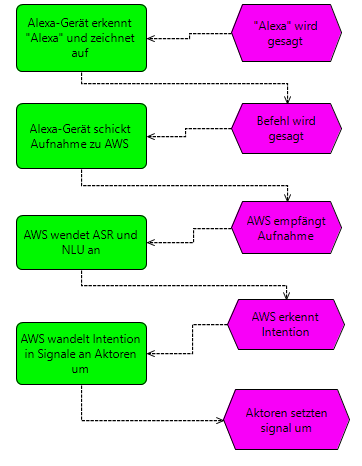
\includegraphics[scale=1]{alexa-epc}
	\caption*{\footnotesize{Quelle: Eigene Darstellung.}}
	\label{fig:alexa_epc}
\end{figure}

So können Befehle an ein Alexa Gerät weitergeben werden, welche über \ac{AWS}, Amazons Cloud, mit beliebigen Aktion verknüpft werden können.
Bspw. kann der Befehl \glqq Alexa, mach mir einen Kaffee.\grqq \ über \ac{AWS} mit der \ac{IoT}-Steuerung einer Kaffeemaschine so verknüpft werden, dass diese dann einen Kaffee produziert.
\autoref{fig:alexa_epc} zeigt die ereignisgesteuerte Prozesskette eines Alexa Sprachbefehls.
Die Verknüpfung von Befehl und Aktion über Alexa wird als \glqq Alexa Skill\grqq bezeichnet.
Zusätzlich gibt es \glqq Alexa Routines\grqq, welche keine Benutzereingaben entgegennehmen, also Automatisierungen darstellen können.

Mit Alexa Skills und Routines können Steuerungsebene, aber auch Automatisierungsebene eines Smart Home Systems realisiert werden.\myfootcite[Vgl.][]{alexa_skills_kit}

\begin{wrapfigure}{r}{0.35\textwidth}
	\centering
	\caption{Works with Alexa Siegel}
	
\includegraphics[scale=.5]{works-with-alexa}
	\caption*{\footnotesize{Quelle: \mycite{figure_works_with_alexa}}}
	\label{fig:works_with_alexa}
\end{wrapfigure}

Smart Home Produkte werden über das Internet mit Alexa verbunden.
Über Skills oder manuelle Programmierung kann ein Gerät, sofern es über ein öffentliches \ac{API} verfügt, angebunden werden.
Um diesen Prozess noch weiter zu vereinfachen können Hersteller die Zertifizierung \glqq Works with Alexa\grqq \ für ihre Produkte erlangen, wenn Spezifikationen bzgl. Installation des Produkts, sowie dessen Schnittstelle erfüllt werden.
\autoref{fig:works_with_alexa} zeigt das Works with Alexa Siegel, welches bei erfolgreicher Zertifizierung benutzt werden darf.
Für Besitzer von zertifizierten Geräten gibt es meist nur noch ein kurzen standardisierten Einrichtungsprozess zu überwinden.\myfootcite[Vgl.][]{workswithalexa}

Amazon Alexa zeichnet sich primär durch die einfache Handhabung aus.
Für die Nutzung und Einrichtung eines Amazon Alexa Systems sind lediglich technische Grundverständnisse bzgl. Smartphones und Computer notwendig.
Dies wird vor allem durch ansprechende Benutzeroberflächen, die direkte sprachliche Kommunikation und zertifizierten Smart Home Produkten ermöglicht.
Auch die Anschaffung eines Alexa Systems ist durch Amazons E-Commerce Plattform einfach.

Aufgrund der zentralen Architektur des Amazon Alexa Systems ergeben sich jedoch auch Probleme.
Wird etwa die Verbindung zum Internet, miteinhergehend die Verbindung zu Amazons Rechenzentrum, unterbrochen kann das Smart Home nicht mehr gesteuert werden, Automatisierungen fallen aus und selbst die Verbindung der einzelnen Smart Home Produkte untereinander sind nicht mehr vorhanden.
Ebenso werden sämtliche Daten durch \ac{AWS} geleitet und nicht lokal gespeichert.
So setzt man die eigenen Daten dem Internet aus.
Ein lokales Speichern und Verarbeiten würde einem Angreifer zunächst die Herausforderung stellen das lokale Heimnetzwerk zu penetrieren.
Dazu wird der Quelltext von Amazon Alexa nicht veröffentlicht und es kann somit nicht nachvollzogen werden, wie die eigenen Daten verarbeitet werden und welche Sicherheitslücken evtl. bestehen.

\subsubsection{Home Assistant}

Home Assistant ist eine Open-Source-Software für Heimautomatisierung.
Durch den modularen Aufbau der Software können Entwickler einfach neue Smart Home Produkte implementieren.
So sind aktuell 1187 Smart Home Produkte über 46 Kategorien mit Home Assistant nutzbar.\myfootcite[Vgl.][]{hass_components}

\begin{figure}[ht]
	\centering
	\caption{Home Assistant Core Architektur}
	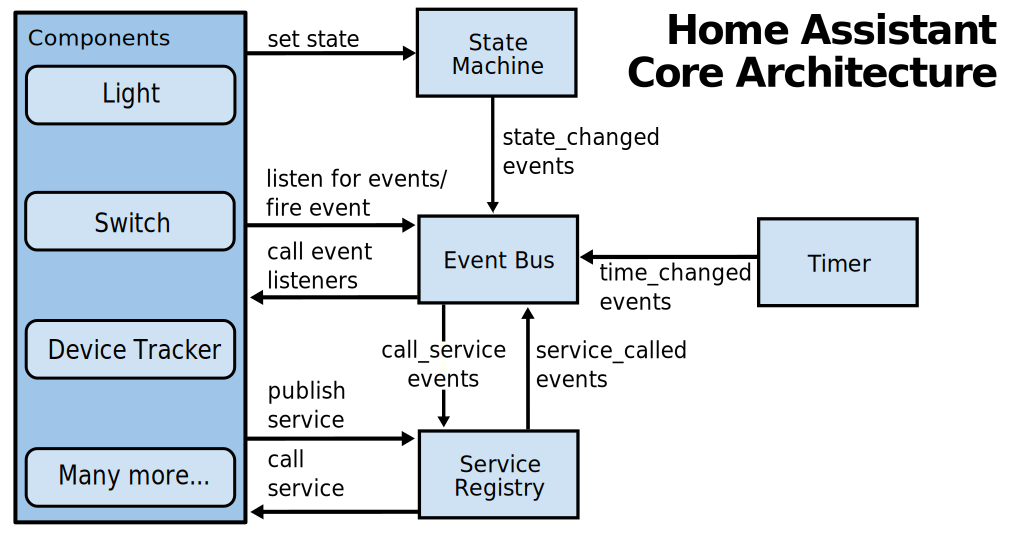
\includegraphics[width=0.9\textwidth]{hass_architecture}
	\caption*{\footnotesize{Quelle: \mycite{hass_architecture_figure}}}
	\label{fig:hasscorearch}
\end{figure}

\autoref{fig:hasscorearch} zeigt die Architektur, welche Home Assistant die Modularität verleiht.
Smart Home Produkte werden als Komponenten implementiert, welche mit dem Home Assistant Core interagieren.
Der Home Assistant Core besteht aus vier Modulen:

Das State Machine Modul bildet den Status der verschiedenen Komponenten ab.
Bemerkt ein Fenstersensor z.B. dass ein Fenster geöffnet wurde, aktualisiert die Komponente \textit{Fenstersensor} ihren Status im State Machine Modul, indem sie eine Nachricht an das Modul schickt.

Für zeitbasierende Automatisierungen existiert das Modul Timer, welches sekündlich ein Event emittiert.
Ein Event ist eine Nachricht, welche beim Auftreten von definierten Bedingungen automatsich verschickt wird.

Über das Event Bus Modul werden Events von den beiden bereits genannten Modulen empfangen von diesen ausgehend wiederum Events ausgelöst.

Das Service Registry Modul bietet Komponenten die Möglichkeit beim Gesamtsystem einen Service zu registrieren.
Das Gesamtsystem wiederum kann über das selbe Modul den Service einer Komponente in Anspruch nehmen.
So kann eine Glühbirne z.B. den Service \textit{Glühbirne anschalten} registrieren, welcher dann von einer anderen Komponente, z.B. einem Lichtschalter, indirekt, über ein Event, aufgerufen werden kann.

Mit dieser Architektur kann eine neue Komponente implementiert werden, ohne dass der Home Assistant Core berührt wird.
Eine neue Komponente muss lediglich einen Service registrieren, auf ein Event reagieren oder ein Event auslösen können.\myfootcite[Vgl.][]{hass_architecture}
Die Implementierung einer neuen Komponente ist ausführlich in der Home Assistant Dokumentation beschrieben.\myfootcite[Vgl.][]{hass_implement_component}

Veröffentlicht wird Home Assistant unter der Apache 2.0 Lizenz.\myfootcite[Vgl.][]{hass_license}
Die Software ist also kommerziell und privat kostenlos nutzbar.
Lediglich die Marke Home Assistant wird geschützt, sowie die Haftung und die Garantie ausgeschlossen.

Für die Weiterentwicklung von Home Assistant wurden im September 2018 vier Grundsätze definiert\myfootcite[Vgl.][]{hass_vision}:

\begin{itemize}
	\item Privatsphäre - alle Daten werden lokal verarbeitet und gespeichert.
	\item Lokale Kontrolle - es ist kein Internetanschluss notwendig.
	\item Offener Quelltext - die Funktionsweise kann jederzeit nachvollzogen werden.
	\item Interoperabilität - es soll einfach sein Apps mit Home Assistant zu verbinden
\end{itemize}

Ebenso wurde Nabu Casa Inc., als Modell für die Finanzierung der Entwicklung von Home Assistant, vorgestellt.
Home Assistant Nutzer können ihre private Instanz mit Nabu Casa um die Home Assistant Cloud Komponente für 5 USD pro Monat erweitern, was Home Assistant \ac{IoT}-Charakter verleiht.
Nabu Casa setzt dazu Software mit offenem Quelltext ein, verspricht keine Daten zu speichern und stellt dem Projekt Home Assistant Entwicklungkapazitäten zur Verfügung.\myfootcite[Vgl.][]{nabucasa}

Mit Home Assistant lassen sich hohe Kosten für zertifizierte Geräte sparen.
Während andere Smart Home System Anbieter, wie z.B. Amazon Alexa, Geräteherstellern die Implementierung von geeigneten Schnittstellen vorschreiben, damit die Geräte mit der jeweiligen Plattform genutzt werden können\myfootcite[Vgl.][]{workswithalexa}, bietet Home Assistant viele verschiedene Wege ein Geräte zu verbinden.
So sind über 1000 Schnittstellen bereits in Home Assistant implementiert\myfootcite[Vgl.][]{hass_components} und zusätzlich können neue oder eigen gebaute Geräte mit neuen Schnittstellen mit etwas Programmierkenntnissen selbst implementiert werden.\myfootcite[Vgl.][]{hass_implement_component}

\begin{wrapfigure}{r}{0.4\textwidth}
	\centering
	\caption{ESP8266 Board}
	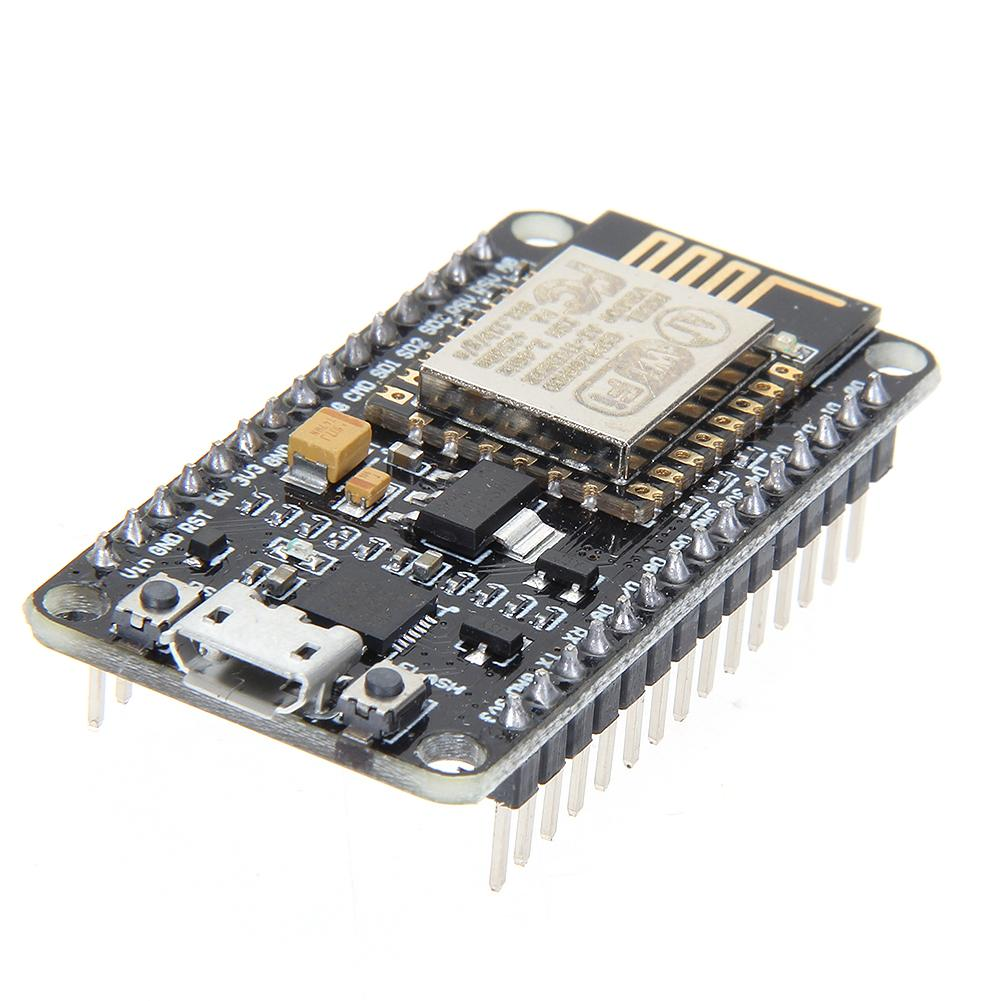
\includegraphics[width=0.4\textwidth]{esp8266}
	\caption*{\footnotesize{Quelle: \mycite{esp8266}}}
	\label{fig:esp8266}
\end{wrapfigure}

\autoref{fig:esp8266} zeigt einen ESP8266 WLAN Mikrocomputer.
In Kombination mit einem Netzteil und Sensoren für Temperatur, Licht und Bewegung kann so eine \ac{DIY}-Wetterstation für weniger als zehn Euro gebaut werden.\myfootcite[Vgl.][]{bruhautomation_esp_sensor}

Der offene Quelltext von Home Assistant ermöglicht zudem, dass jederzeit nachvollzogen werden kann, was mit den eigenen Daten passiert.
Außerdem funktioniert Home Assistant vollständig offline.
Bei einem Internetausfall bleibt das Smart Home also weiter nutzbar.
Gleichzeitig bedeutet das auch, dass Dritte sich erst Zugriff zum eigenen Heimnetzwerk verschaffen müssen, damit ein Versuch unternommen werden kann Daten zu kompromittieren.

Zusammenfassend bietet Home Assistant Privatsphäre, Unabhängigkeit gegenüber des Internets, sowie eine hohe Bandbreite an verfügbaren Geräten und nutzbaren Schnittstellen.

Home Assistant wird von einer \glqq worldwide community of tinkerers and DIY enthusiasts.\grqq{}\myfootcite{hass_github_organization} entwickelt.
Gleichermaßen richtet sich Home Assistant als Produkt auch an Bastler und Tüftler.
So müssen Englischkenntnisse und Erfahrung im Umgang mit Linux und Computernetzwerken für die Einrichtung von Home Assistant vorhanden sein.\myfootcite[Vgl.][]{hass_getting_started}

Zudem befindet sich Home Assistant noch in aktiver Entwicklung und so fordern manche Änderungen der Software aktive Maßnahmen des Benutzers, wie etwa das Aktualisieren einer Konfigurationsdatei.\myfootcite[Vgl.][]{hass_breaking_change_example}

Home Assistant kann im jetzigen Zustand nur von technisch Versierten genutzt werden.

\subsubsection{HomeMatic IP}

Unter der Marke HomeMatic IP vertreibt die deutsche Aktiengesellschaft eQ-3 eine Smart Home Komplettlösung, welche die Bereiche Heizung und Klima, Sicherheit und Alarm, Licht und Schatten, sowie Wetter und Umwelt bedient.
\myfootcite[Vgl.][19f]{eq3_homematicip_docs}

\begin{figure}[ht]
	\centering
	\caption{HomeMatic IP Geräte}
	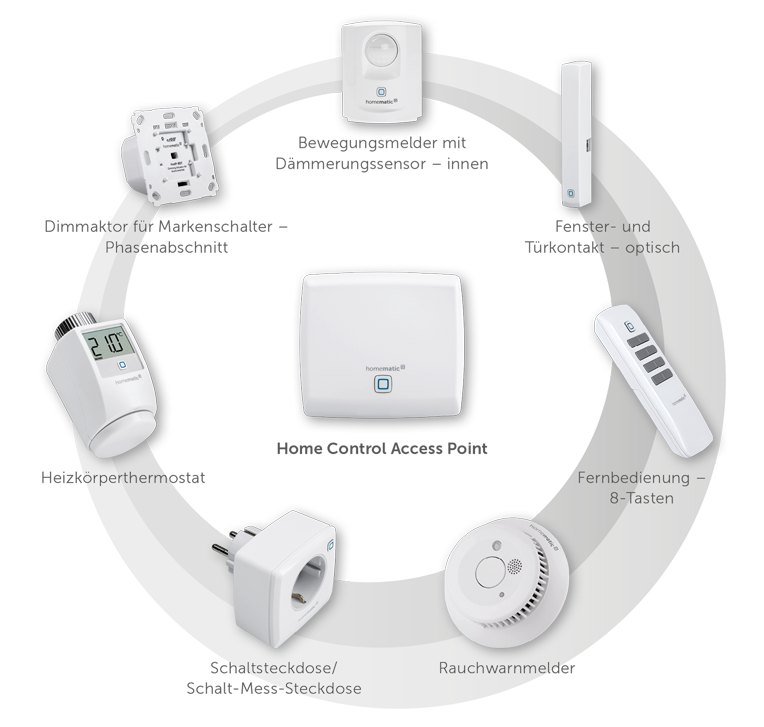
\includegraphics[width=0.9\textwidth]{homematic-star}
	\caption*{\footnotesize{Quelle: \mycite{figure_homematicip}}}
	\label{fig:homematic_star}
\end{figure}

Bei HomeMatic IP werden einzelne Smart Home Geräte direkt, wie in einer Stern-Netzwerk-Topologie, über das 868 MHz Band mit einem Hub - dem HomeMatic IP Access Point - verbunden.
Der Hub wiederum wird über das Internet mit einer Cloud - der HomeMatic IP Cloud - verbunden, welche die Automatisierung und die Steuerung des Smart Home Systems übernimmt.
Über die HomeMatic IP Smartphone App, aber auch Sprachassistenten von Google oder Amazon, kann das Gesamtsystem manuell gesteuert werden.
\autoref{fig:homematic_star} zeigt HomeMatic IP Produkte, welche direkt mit dem HomeMatic IP Access Point verbunden werden müssen.
Eine Internetverbindung ist bei der Installation des Systems zwingend notwendig.
Ist das HomeMatic IP System eingerichtet kann teilweise auch auf eine Internetverbindung verzichtet werden, so werden direkte Verknüpfungen zwischen einzelnen Smart Home Geräten erkannt und lokal abgespeichert.\myfootcite[Vgl.][22-25]{eq3_homematicip_docs}

Soll ein Smart Home System mit \ac{IoT}-Charakter an Konsumenten mit durchschnittlichem technischen Verständnis empfohlen werden, dann überzeugt HomeMatic IP vor allem durch Datenschutz.
eQ-3 gibt an Daten ausschließlich anonymisiert auf deutschen Servern abzuspeichern.
Außerdem müssen bei der Einrichtung eines HomeMatic IP Systems keine persönlichen Daten angegeben werden.\myfootcite[Vgl.][24]{eq3_homematicip_docs}
Auf technischer Ebene ist hervorzuheben, dass auf dem 868 MHz Band operiert wird, was eine Kommunikation frei von Interferenzen ermöglicht.\myfootcite[Vgl.][18]{eq3_homematicip_docs}
Des Weiteren stellt eQ-3 durch automatische \ac{OTA}-Aktualisierungen sicher, dass die HomeMatic IP Geräte stets auf dem aktuellensten Sicherheitspatchlevel sind.
Schließlich ist das HomeMatic IP Ökosystem auch für andere Gerätehersteller offen.\myfootcite[Vgl.][]{eq3_faq}
Zudem bieten über 100 eQ-3-Partner deutschlandweit die professionelle Einrichtung oder Unterstützung bei der Einrichtung eines HomeMatic IP Systems an, was die Barriere auf dem Weg zum Smart Home System für normale Konsumenten herabsetzt.\myfootcite[Vgl.][]{eq3_haendler}

Wie bei den meisten Smart Home Systemen ist jedoch anzumerken, dass eine Abhängigkeit zur Cloud besteht.
Bei einem Internetausfall kann das Smart Home nicht mehr per Smartphone App gesteuert werden.
Außerdem ist die, auf aktuell ca. 80 Produkte limitierte, geringe Angebotsbreite zu beachten.\myfootcite[Vgl.][]{eq3_product_count}

\subsection{Geschäftsmodelle}

Die Smart Home Industrie wird sich mit rasantem Wachstum konfrontiert sehen.
\autoref{tab:smarthome_market_predictions} zeigt verschiedene Vorhersagen für zukünftige Marktvolumina.
Bei Betrachtung des geschätzten Marktvolumens von 39,68 Mrd. USD nach Mordor Intelligence \myfootcite[Vgl.][]{market_mi} in 2017, ist eine klar optimistische Tendenz zu erkennen.

\begin{table}[ht]
	\caption{Smart Home Marktvolumen Vorhersagen}
	\centering
	\begin{tabular}{| p{0.3\textwidth} | p{0.2\textwidth} | p{0.3\textwidth} |}
		\hline
		\textbf{Institut} 	& \textbf{Jahr} & \textbf{Marktvolumen} \\ \hline
		Ironpaper & 2020 & 58,58 Mrd. USD \\ \hline
		Zion Market Research & 2022 & 53,45 Mrd. USD \\ \hline
		Market Research Future & 2023 & 137,95 Mrd. USD \\ \hline
		Mordor Intelligence & 2023 & 159,68 Mrd. USD \\ \hline
	\end{tabular}
	\caption*{\footnotesize{Quellen: \mycite[Vgl.][]{market_ironpaper,market_mrf,market_zmr,market_mi}}}
	\label{tab:smarthome_market_predictions}
\end{table}

Nachfolgend werden beispielhaft Geschäftsmodelle erklärt, welche dem erkannten Trend beitragen und beitragen werden.

\subsubsection{Smart Home Geräte}

Bei Betrachtung der Schätzungen in \autoref{tab:smarthome_market_predictions} ist die Idee des Verkaufs von \ac{IoT}-Geräte für Smart Homes so naheliegend, wie Schaufeln während eines Goldrausches zu verkaufen.
Schenkt man den Zahlen von Mordor Intelligence Glauben kann von einem Marktwachstum von ca. 300\% über die nächsten sechs Jahre ausgegangen werden, was einer jährlichen Wachstumsrate von ca. 20\% entspricht.

Beim Verkauf von \ac{IoT}-Geräte für Smart Homes können verschiedene Ansätze gewählt werden.
Es kann sich dafür entschieden werden das zu verkaufende Produkt zertifizieren zu lassen.
Standards wie ZigBee, Z-Wave oder Works with Alexa ermöglichen es das Produkt einfacher zu vermarkten, da potentielle Kunden die einfachere Interoperabilität schätzen.
Nicht zu unterschlagen ist jedoch, dass eine solche Zertifizierung, je nach Marke, mit Kosten verbunden ist, in Form von Entwicklungskosten und Kosten für die Zertifizierung.
Die Zertifizierung eines ZigBee Produktes kostet z.B. 1000 USD.\myfootcite[Vgl.][]{zigbee_certification}
Alternativ kann das Produkt unter einer Eigenmarke vertrieben werden um genannte Kosten zu minimieren, was jedoch erhöhte Marketingkosten bedingt.
Zudem ist zusätzlich eine Cloud-Infrastruktur zu unterhalten, über welche die Kunden ihr Produkt steuern.
Bei einer Zertifizierung, bzw. der Integration in ein bereits vorhandenes Ökosystem fallen diese Kosten weg.
Schließlich bleibt noch die Option das Produkt mit offener \ac{API} und einer Dokumentation für Bastler, bzw. offline Smart Homes zu verkaufen, für welche eine Integration in ein \ac{IoT}-Smart Home System überflüssig wäre.

Nach Splendid Research interessierten sich in 2017 76,1\% der Deutschen für das Thema Smart Home.\myfootcite[Vgl.][]{smart_home_2017_de}
Bei ca. 42 Millionen Wohnungen in Deutschland  wären also mindestens ca. 32 Millionen Wohnende in Deutschland an Smart Home Produkten interessiert.\myfootcite[Vgl.][]{destatis_wohnungen_in_de_2017}

\subsubsection{Systemanbieter}

Die Installation von Smart Home Systemen ist aufgrund der verschiedenen Standards und Schnittstellen von Smart Home Geräten nicht trivial.
Zudem kommt erschwerend hinzu, dass meist ein individuelles System installiert werden muss,  von verschiedenen Bewohnerpräferenzen und Architekturgegebenheiten.
Außerdem besteht Bedarf an grundlegendem technischen Verständnis.
So erscheint es logisch \glqq Smart-Home-as-a-Service\grqq \ anzubieten.
Dabei erstreckt sich die Dienstleistung von der Konzeption eines Smart Home Systems, egal ob bei Neu- oder Altbau, über die eigentliche Installation des Systems, bis hin zur Wartung und Aktualisierung des installierten Systems.

\begin{table}[ht]
	\caption{Smartest Home Produktkatalog}
	\centering
	\begin{tabular}{| p{0.3\textwidth} | p{0.3\textwidth} |}
		\hline
		\textbf{Produkt} & \textbf{Preis} \\ \hline
		Basic & ab 15.000 Euro/CHF \\ \hline
		Komfort & ab 30.000 Euro/CHF \\ \hline
		Premium & ab 60.000 Euro/CHF \\ \hline
		High-End & ab 150.000 Euro/CHF \\ \hline
		Luxus & auf Anfrage \\ \hline
		Nachrüstung & auf Anfrage \\ \hline
	\end{tabular}
	\caption*{\footnotesize{Quellen: \mycite[Vgl.][]{smartesthome_website}}}
	\label{tab:smartesthome_products}
\end{table}

\autoref{tab:smartesthome_products} zeigt den Produktkatalog von Smartest Home, einem Smart Home Systemanbieter.
Smartest Home verspricht für die Preise in \autoref{tab:smartesthome_products} \glqq die gesamte Konzeption und Planung, [zu] helfen bei der Produkteauswahl und [...] einzusetzende Schaltschränke fixfertig für den Elektriker [zu programmieren].\grqq{} \myfootcite{smartesthome_yoursmarthome}

Da hier Wissen verkauft wird, was der Systemanbieter sich nur einmal aneignen muss entsteht bei einem Neuauftrag nur ein minimaler Aufwand.
So kann von einer hohen Marge ausgegangen werden.
Nach Splendid Research nutzten ca. 36\% der Deutschen in 2017 bereits Smart Home Systeme und weitere 40\% interessierten sich für Smart Home Systeme.\myfootcite[Vgl.][]{smart_home_2017_de}
Überträgt man dies auf die ca. 200.000 jährlich neu gebauten Wohnungen in Deutschland, werden etwa 72.000 Smart Home Systeme allein in Deutschland jährlich installiert.\myfootcite[Vgl.][]{baufertigstellungen}
Außerdem würden sich weitere 80.000 Wohnungsbesitzer für Smart Home Systeme interessieren.
Würden nur 1\% der jährlich vorgenommen Smart Home Installationen durch professionelle Systemanbieter durchgeführt werden blieben immer noch 720 Smart Home Installationen pro Jahr.

\subsubsection{Fernsteuerungs-Dienst}

Aus Bedenken, wie dem Verlust der Kontrolle über die Steuerung eines Smart Home Systems, werden manche Smart Home Systeme bewusst nicht mit dem Internet verbunden.
Unabhängig davon besteht aber weiterhin das Interesse an der Fernsteuerung des Smart Home Systems.
Oft wird eine solche Fernsteuerung dann über einen \ac{VPN}-Zugang so realisiert, dass man sich mit dem Smartphone mit dem eigenen Heimnetzwerk verbindet und dann das Smart Home System über eine Web-Oberfläche steuert.
Dabei muss jedoch ein kleiner Heimserver installiert werden, welcher den \ac{VPN}-Zugang hostet und einen dynamischen \ac{DNS}-Dienst anspricht um die aktuelle IP-Adresse des Smart Homes nach außen bekannt zu machen.
Das Betreiben des Servers bringt ein Hardware- und Zeitinvestment, sowie laufende Kosten mit sich.
Fernsteuerungs-Dienste minimieren den Einrichtungsprozess, verbessern das Benutzererlebnis und weisen meist auch geringere laufende Kosten auf, wofür der Smart Home Bewohner zahlungsbereit ist.

Das Unternehmen Nabu Casa bietet bspw. unter dem Produktnamen \ac{HAC} einen Fernsteuerungs-Dienst für Home Assistant an.
Monatlich werden hier 5 USD verlangt.
Dafür wird nicht nur die eigene Home Assistant Instanz fernsteuerbar, sondern auch die Schnittstelle geboten um Home Assistant mit Amazon Alexa oder Google Assistant zu steuern.
Dabei fungiert die \ac{HAC} als reiner Übertragungdienst.
So übersetzt sie lediglich die Eingaben des Smart Home Bewohners, egal ob über App oder Sprachassistent, in ein für Home Assistant lesbares Format und schickt diese an die Home Assistant Instanz, welche fortfolgend die entsprechenden Aktoren ansteuert.
Hier wird auch klar, dass die Nutzung von \ac{HAC} einen Gewinn an Sicherheit bedeutet, da nicht wie herkömmliche über einen \ac{VPN} Vollzugriff auf das eigene Heimnetzwerk vergeben werden muss.\myfootcite[Vgl.][]{nabucasa}

Das Geschäftsmodell ist zwar wirtschaftlich, nicht aber von großer monetärer Relevanz.
Zum Zeitpunkt dieser Arbeit existieren ca. 30.000 Home Assistant Instanzen (geschätzt unter Berücksichtigung der Anzahl an Sternen des Projekts auf GitHub).
Auch bestehen neben Home Assistant keine relevanten Smart Home Systeme, welche ohne Internetzugang betrieben werden können.

\subsubsection{Standard}

Eine weitere Möglichkeit den Smart Home Markt zu monetarisieren besteht in der Etablierung eines Standards.
Bei der Entwicklung von Smart Home Produkten ist die Interoperabilität und die Schnittstellendefinition kritisch für die Adaption des Produkts.
So erleichtert sich die Kaufentscheidung für ein Smart Home Produkt bspw., wenn ein Amazon Alexa Logo die Kompatibilität mit den bereits daheim installieren Alexa Produkten garantiert.
Außerdem minimiert die Nutzung eines Standards bei der Implementierung eines Kommunikationssystems in ein Smart Home Produkt die geforderte technische Kompetenz auf die Fähigkeit einem Implementierungshandbuch Folge leisten zu können.

So überrascht es nicht, dass bereits über 94 Millionen Z-Wave Geräte\myfootcite[Vgl.][]{zwave_products_sold}, über 500 Millionen ZigBee Geräte\myfootcite[Vgl.][]{zigbee_devices_sold} und über 10 Millionen Amazon Alexa Geräte\myfootcite[Vgl.][]{alexa_devices_sold} verkauft wurden.

Über den Verkauf des Zugangs zu Implementierungsunterlagen, die Zertifizierung von neuen Produkten oder über Gebühren für die generelle Li­zen­zie­rung des jeweiligen Standards konnten die bereits existierenden Anbieter von Smart Home Standards bereits profitieren.

\subsubsection{Integrierte Einkäufe}

In einem normalen Haushalt müssen regelmäßig Verbrauchsgüter wie Klopapier, Waschmittel oder Lebensmittel eingekauft werden.
Durch die Integration sämtlicher Haushaltsgeräte in ein Smart Home System kann der Bedarf der verschiedenen Verbrauchsgüter leicht erfasst werden.
So kann die Beschaffung der benötigten Verbrauchsgüter über automatisierte Bestellungen bei Plattformen wie z.B. Amazon vollständig automatisiert werden, was ökonomisch und ökologisch ungünstigere Einkäufe bei lokalen Supermarktketten erspart.
Die Einrichtung solcher integrierter Einkäufe erfolgt über das Smart Home System, welchem auch die explizite Produktauswahl überlassen wird.
So kann der Smart Home Anbieter die Nachfrage der Smart Home Nutzer an Verbrauchsgüterhersteller versteigern und dabei mit an dem Konsum der Smart Home Nutzer verdienen.

Darüber hinaus können auch Softwarekomponenten verkauft werden, welche die vorhandenen Automatisierungen oder Steuerungen ergänzen oder verbessern.
So verkauft der Software Entwickler Jeff Bolton eine Premiumversion seines Alexa Skills \glqq Sleep and Relaxation Sounds\grqq{}, welche Nutzern beim Einschlafen und Entspannen hilft, mit einer Konversionsrate von 43\%, was eine hohe Zahlungsbereitschaft für bessere Integrationen, Automatisierungen und Dienstleistungen innerhalb des eigenen Smart Homes erkennen lässt.\myfootcite[Vgl.][]{alexa_inskill_purchase}

Das Smart Home System Amazon Alexa bietet bereits die Möglichkeit die beschriebenen integrierten Einkäufe sogar per Sprachbefehl einzurichten, bzw. durchzuführen, was alle Amazon Alexa Nutzer zu potentiellen Kunden für integrierte Einkäufe macht.\myfootcite[Vgl.][]{alexa_making_money_with_skills}

\section{Fazit}

Nach über 50 Jahren Smart Home Spielereien sind in den letzten 10 Jahren, im Aufkommen des \ac{IoT}, Geschäftsmodelle und Produkte im Smart Home Bereich entstanden, welche erfolgreich einen stark wachsenden Smart Home Markt etabliert haben.
Vor allem der Erfindung des Smartphones hat der heutige und zukünftige Smart Home Markt zu danken.
Aufgrund der Vernetzung der Menschen durch Smartphones wurde der Mehrwert der Vernetzung von Maschinen erst greifbar.
Spätestens mit der Markteinführung von Amazon Alexa in 2012 wurde der Smart Home Trend global ausgelöst.

Heute versteht man unter einem Smart Home ein System, welches durch Automatisierungen das Leben in einem Gebäude einfacher macht, aber auch Möglichkeiten zur bequemen Steuerung und Überwachung des Gebäudes und dessen Geräte bietet.
Dabei wird in nahezu jedem neu installierten Smart Home System dazu tendiert \ac{IoT}-Komponenten zu verbauen.
Dies stellt ein Problem dar.
Viele \ac{IoT}-Produkthersteller implementieren \ac{IoT}-Funktionalitäten in ihre Produkte ohne sich über die Sicherheit ihrer Produkte Gedanken zu machen und darüber hinaus liefern die wenigstens Hersteller Sicherheitsaktualisierungen aus, falls eine Sicherheitslücke in ihrem Produkt bekannt wird.
Langfristig wird sich kein Hersteller mit einer solchen Einstellung halten können, was eine positive Veränderung bzgl. Sicherheit von \ac{IoT} und Smart Home Produkten impliziert.
Bis diese Veränderung eintritt ruft der Twitter-Benutzer und \ac{IoT}-Kritiker \glqq Internet of Shit\grqq{} Konsumenten dazu auf, sich genau zu überlegen, welche \ac{IoT}-Produkte den Haushalt wirklich vereinfachen und nur diese zu kaufen, um nicht ohne Mehrwert eine potentielle Sicherheitslücke in Kauf zu nehmen.\myfootcite[Vgl.][]{internet_of_shit}
Aus Datenschutzsicht wäre es sogar noch besser, wenn das hauseigene Smart Home System gar nicht, oder nur über genau eine kontrollierte Schnittstelle mit dem Internet kommunizieren würde.
Gerade weil die meisten Hersteller von Smart Home Produkten den Quelltext der Software ihrer Produkte nicht veröffentlichen und somit nicht sichergestellt werden kann, was mit den eigenen Daten passiert und welche Abhängigkeiten bestehen, sollte eine offline Smart Home Lösung, wie z.B. Home Assistant immer vorgezogen werden.

Aktuell ringen sich Smart Home Standards, wie ZigBee, Z-Wave und Amazon Alexa darum die einzige Plattform für Smart Homes zu werden.
Noch ist unklar, welcher Standard sich durchsetzen wird.
Nach dem Metcalfeschen Gesetz steigert sich der Nutzen eines Netzwerks quadratisch zur Anzahl der Nutzer des Netzwerks.\myfootcite[Vgl.][184]{informationrules}
So wird auch der Standard mit dem größten Produktportfolio und den meisten Nutzern den aktuellen Standard-Krieg höchstwahrscheinlich gewinnen.
Gibt es einen eindeutig vorherrschenden Smart Home Standard können sich Konsumenten einfach mit Smart Home Produkten ausstatten, ohne dass auf eine passende Plattformintegration geachtet werden muss, was den Nutzen von vernetzen Smart Home Geräten nach Metcalfe's Gesetz noch schneller steigern wird.

\begin{figure}[ht]
	\centering
	\caption{Google Trends zu Künstliche Intelligenz}
	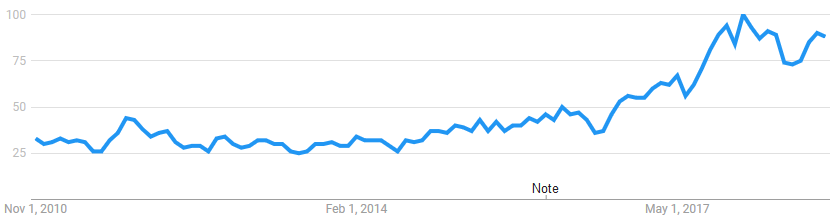
\includegraphics[width=0.9\textwidth]{ai-google-trends}
	\caption*{\footnotesize{Quelle: \mycite{google_trends_ai}}}
	\label{fig:googletrends_ai}
\end{figure}

Des Weiteren ist denkbar, dass zukünftig die aktive Kontrolle über ein Smart Home in den Hintergrund rückt und an eine künstliche Intelligenz abgegeben wird, welche die Intentionen der Bewohner nicht nur über Sprachbefehle interpretiert, sondern auch Verhaltensmuster und persönliche Daten analysiert.
\autoref{fig:googletrends_ai} zeigt dazu die steigende Relevanz von künstlicher Intelligenz.

Auch die Versicherungsbranche könnte mit in Smart Homes involviert werden, indem z.B. Versicherungsprämien reduziert werden, beim Einsatz von mit dem Versicherer vernetzten Sicherheitssysteme.\myfootcite[Vgl.][]{smart_home_future}

Letztendlich bleibt unklar wie sich der Alltag mit Smart Homes in Zukunft gestalten wird und es können nur Vermutungen angestellt werden, ähnlich wie bei der Entwicklung des Internets selbst.